\documentclass{book}
\usepackage[utf8]{inputenc}
\usepackage{ bussproofs }
\usepackage{ amssymb }
\usepackage{hyperref}
\usepackage{listings}
\usepackage{xargs}
\usepackage{simplebnf}
\usepackage{float}
\usepackage{xcolor}
\usepackage{numprint}
\usepackage{ amsmath }
\usepackage{mathpartir}
\usepackage{minted}
\usepackage[hashEnumerators,smartEllipses, hybrid]{markdown}
\usemintedstyle{monokai}
\usepackage{amsthm}
\usepackage{csquotes}
\usepackage[british]{babel}

\usepackage[bibstyle=numeric, backend=bibtex, sorting=none]{biblatex}
\addbibresource{../Meine Bibliothek.bib}

\usepackage{draculatheme}


\usepackage[colorinlistoftodos,prependcaption,textsize=tiny]{todonotes}

\newcommandx{\unsure}[2][1=]{\todo[linecolor=red,backgroundcolor=red!25,bordercolor=red,#1]{#2}}
\newcommandx{\change}[2][1=]{\todo[linecolor=blue,backgroundcolor=blue!25,bordercolor=blue,#1]{#2}}
\newcommandx{\info}[2][1=]{\todo[linecolor=OliveGreen,backgroundcolor=OliveGreen!25,bordercolor=OliveGreen,#1]{#2}}
\newcommandx{\improvement}[2][1=]{\todo[linecolor=Plum,backgroundcolor=Plum!25,bordercolor=Plum,#1]{#2}}
\newcommand{\code}[1]{\texttt{#1}}

\newcommand{\mtext}[1]{$\text{#1}$}
\newcommand{\tuple}[2]{\langle #1 \mid #2 \rangle}


\newcommand{\ccolon}[0]{: }
\newcommand{\cmid}[0]{| }
\newcommand{\cdisj}[0]{|| }


\newtheorem{theorem}{Theorem}[section]
\newtheorem{corollary}{Corollary}[theorem]
\newtheorem{lemma}[theorem]{Lemma}
\theoremstyle{definition}
\newtheorem{definition}[theorem]{Definition}

\begin{document}

\tableofcontents


Software correctness is a central goal for software development.
One way to improve correctness is using strong and descriptive types and verifying them with type systems.
In particular Refinement Types demonstrated, that even with a verification system that is restricted to a decidable logic, intricate properties can be expressed and verified in a lightweight and gradual way.
However existing approaches for adapting Refinement Types from functional to imperative languages proved hard without compromising on at least one of core features of Refinement Types.
% I argue that a base language restricted to unique mutable references will make
This thesis aims to design a Refinement Type system without such compromises by taking advantage of Rust's restriction to unique mutable references.
I will define a Refinement Type language and typing rules and argue for their soundness. Additionally I will implement a prototype verifier to evaluate the effectiveness of the approach on selected examples.





\chapter{Introduction}

% With increasing reliance on increasingly complex software, ensuring correctness of programs is a vital concern to software development.
With increasing amount and reliance of software, ensuring the correctness of programs is a vital concern for the future of software development.
Although research in this area has made good progress, most approaches are not accessible enough for general adoption by the developers. Especially in light of a predicted shortage of developers\cite{breaux_2021_2021-1}, it is not sufficient to require developers to undergo year-long training in specialized and complex verification methods to ensure the correctness of their software. It is therefore crucial to integrate with their existing tooling and workflows to ensure the future high quality of software.
One avenue for improving accessability for functional verification is extending the expressiveness of the type system to cover more of the correctness properties.
Using type systems for correctness was traditionally prevalent in purely functional languages where evolving states are often represented by evolving types, offering approachable and gradual adoption of verification methods. Tracing evolving states in the type system would be especially useful for languages with mutability, since substantial parts of the behaviour of the program is expressed as mutation of state. In particular Rust seems like a promising target language, because mutability is already tracked precisely and thus promising functional verification for relatively minimal effort on the programmer's part.

The goal of the thesis is to show that Refinement Types can be idiomatically adapted to languages with unique mutable references. The type system presented in this thesis enables gradual adoption of lightweight verification methods in mutable languages.

%In case implementing these translations could not be completed, the use cases will be transformed manually.
The type system is sound and effective in the identified use-cases.
%In addition, a description of the syntax and semantics of the constructs, that will extend Rust's type system, will be provided as well as justification for their soundness. 
A feasibility study on minimal examples of challenging use cases shows how useful the proposed verification system is. 
%For use cases that could not be covered by the proposed additions, the reason will be investigated.

Specifying or verifying complete Rust modules or the entire Rust language is not the goal of the thesis. In particular \code{unsafe} Rust will not be taken into account in specification nor implementation. Implementing Liquid Type inference in also not a goal of the thesis.

The accompanying implementation extends the Rust compiler, enables automatic parsing of the refinement type language and automated type checking of a subset of Rust, as well as limited inference and error reporting. 
The thesis also gives a description of the syntax and semantics of the subset of Rust as well as the refinement type system.

The contributions of this thesis are:
\begin{enumerate}
  \item Automatic empirical analysis of the usage of mutability and unsafe in Rust using syntactic information
  \item Extension to the Rust type system to allow for refinement type specifications
  \item Description and implementation of a type checker for the introduced type system
  \item Evaluation of the type system on minimal benchmarks
\end{enumerate}

The thesis if structured as follows: 
In chapter XXX an empirical analysis of \code{unsafe} and mutability uses is performed. 
Then chapter XXX will give an overview of the foundation the thesis build upon. 
Chapter XXX defines the subset of Rust, that will be the basis for the type system.
Next chapter XXX explains the actual type system and verification, as well as justifying its correctness, followed by chapter XXX, which will provide more information about the implementation.
The type system will then be tested in minimal benchmarks in chapter XXX.
Chapter XXX reports on related work and alternative approaches.
Finally chapter XXX concludes the thesis and gives an overview over possible future work.


\chapter{Empirical Analysis of Use-Cases}

Before designing a system for Rust, it makes sense to gain some understanding of how Rust is used. For this purpose we will look at two key features of Rust, that influence how an approachable verification should look like.
Firstly \code{unsafe} Rust with similar guarantees to C would make verification and specification significantly harder. But if the use of \code{unsafe} is limited, like intended by the language designers, it would allow us to focus on the save part of Rust and leave the verification of \code{unsafe} Rust to more complex verification systems.
Secondly with mutability being the main difference to the traditional domain fof Refinement Types, showing the need for covering this area and to what degree of approachability it interesting.

There are two fundamental assumptions for the usefulness of the type system: 
\begin{enumerate}
  \item \label{enum:hypothesis-unsafe-rare} Uses of \code{unsafe} are rare
  \item \label{enum:hypothesis-unsafe-lib} In the rare case, that \code{unsafe} is used, is is mostly used internally (not exposed to the callee)
  \item \label{enum:hypothesis-mut} Mutability is used pervasively in Rust.
\end{enumerate}

To check these assumptions an analysis of existing Rust code was performed. As a basis for the analysis, the Rust package registry href{https://www.crates.io} was used. It contains the source code for both Rust libraries as well as various applications written in Rust (e.g. ripgrep). 

We analyzed all published Rust crates on February 2nd 2022 (Rust's version packages) on crates.io with at least 10 versions\footnote{The limit of 10 versions is used to eliminate inactive and placeholder packages}, which totals \numprint{11882} crates, containing \numprint{228263} files with a combined code-base size of over 64 million lines of Rust code (without comments and white space lines)\footnote{Calculated with \texttt{cloc}}. 

% from cloc
% ----------------------------------------------------------------------------------------
% Language                              files          blank        comment           code
% ----------------------------------------------------------------------------------------
% Rust                                 228263        5664979       10317162       64193670
% C                                     32945        1539542        1979846       13468919
% C++                                   18084        1263696        1093652        7956897
% JSON                                  15838           1897              0        6424252
% C/C++ Header                          31619        1152322        2015896        6284146
% XML                                    5142          25277          25773        4807556
% Assembly                               4146         534785         582345        2631991

The analysis parses these files and searches for certain patterns, which are subsequently extracted and saved.
Thanks to using the tree-sitter parsing framework, the analysis framework can easily be extended to other queries and languages.

\label{ss:unsafe-rust}\section{Unsafe Rust}

Firstly we will be checking the hypothesis \ref{enum:hypothesis-unsafe-rare}.
There is already some research on how \code{unsafe} is used in Rust. For example Astrauskas et al. \cite{astrauskas_how_2020} found, that about 76\% of crates did not use any unsafe. On top of that, unsafe signatures are only exposed by

"The majority of crates (76.4\%) contain no unsafe features at all. Even in most crates that do contain unsafe blocks or functions, only a small fraction of the code is unsafe: for 92.3\% of all crates, the unsafe statement ratio is at most 10\%, i.e., up to 10\% of the codebase consists of unsafe blocks and unsafe functions." \cite[p. 13]{astrauskas_how_2020}
Our data seems to confirm this: \numprint{8044} of the \numprint{11882} crates (67.7\%) did not use any unsafe. 

Astrauskas et al. also found, that "however, with 21.3\% of crates containing some unsafe statements and – out of those crates – 24.6\% having an unsafe statement ratio of at least 20\%, we cannot claim that developers use unsafe Rust sparingly, i.e., they do not always follow the first principle of the Rust hypothesis." \cite[p. 14]{astrauskas_how_2020}
If this is the case for applications, it might disprove hypothesis hypothesis \ref{enum:hypothesis-unsafe-lib}. 
When checking unsafely for our use case, it makes sense to further distinguish between libraries and executables crates: Libraries are intended to be used by other Rust programs: Usage of unsafe in libraries may not be as problematic as in executables, because libraries are written once but used by many applications, justifying higher verification effort. 

In our analysis we found, that firstly crates.io contains significantly more libraries than binaries\footnote{Libraries and Executables are distinguished by checking if they contain \code{bin} or \code{lib} target or one of the corresponding files according to the cargo naming convention.} (see Figure \ref{fig:crate_types}). 
And secondly libraries are much more likely to use \code{unsafe} Rust. Table shows the result of our analysis. Where uses of \code{unsafe} are counted and grouped by crate type (see Table \ref{tab:unsafe-uses-by-crate}).
The data in the table includes all crates except \code{windows-0.32.0}, which alone contains \numprint{233608} uses of \code{unsafe}. Nearly $2 / 3$ of all other library \code{unsafe} combined.
Looking at the distribution of unsafe uses in Figure \ref{fig:unsafe-hist}, we can see, that this is an exception: Most other libraries do not use that much unsafe statements. We can also see, that even if a executable crate uses \code{unsafe}, it uses few.



\begin{figure}[h]
	\centering
	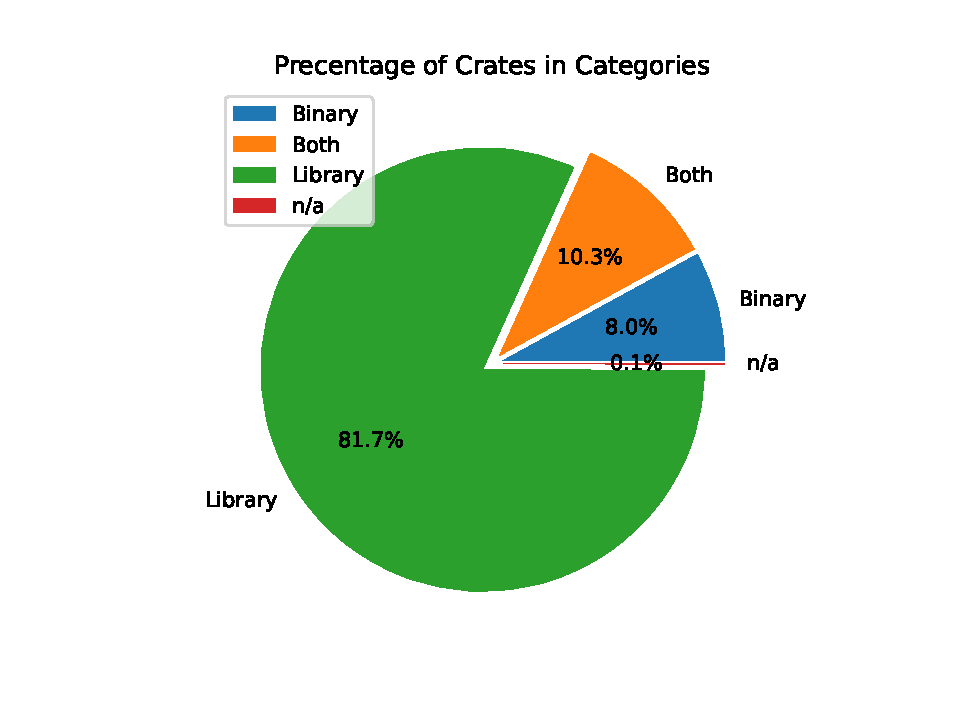
\includegraphics[width=0.7\linewidth, clip, trim={0.5cm 0.5cm 0.5cm 0.5cm}]{../crate_types.pdf}
	\caption{Percentage of Crates, that Contain Libraries, Executables or Both}
	\label{fig:crate_types}
\end{figure}

\begin{table}[h]
\centering
\begin{tabular}{l | r}
  & Number of Unsafe Uses \\
  Crate Type &  \\
  \hline
 Library & \numprint{382997} \\
 Both & \numprint{7720} \\
 Binary & \numprint{930} \\
 n/a & \numprint{215} \\
 \end{tabular}
\caption{Number of Unsafe Uses by Crate Category}
\label{tab:unsafe-uses-by-crate}
\end{table}



\begin{figure}[h]
	\centering
	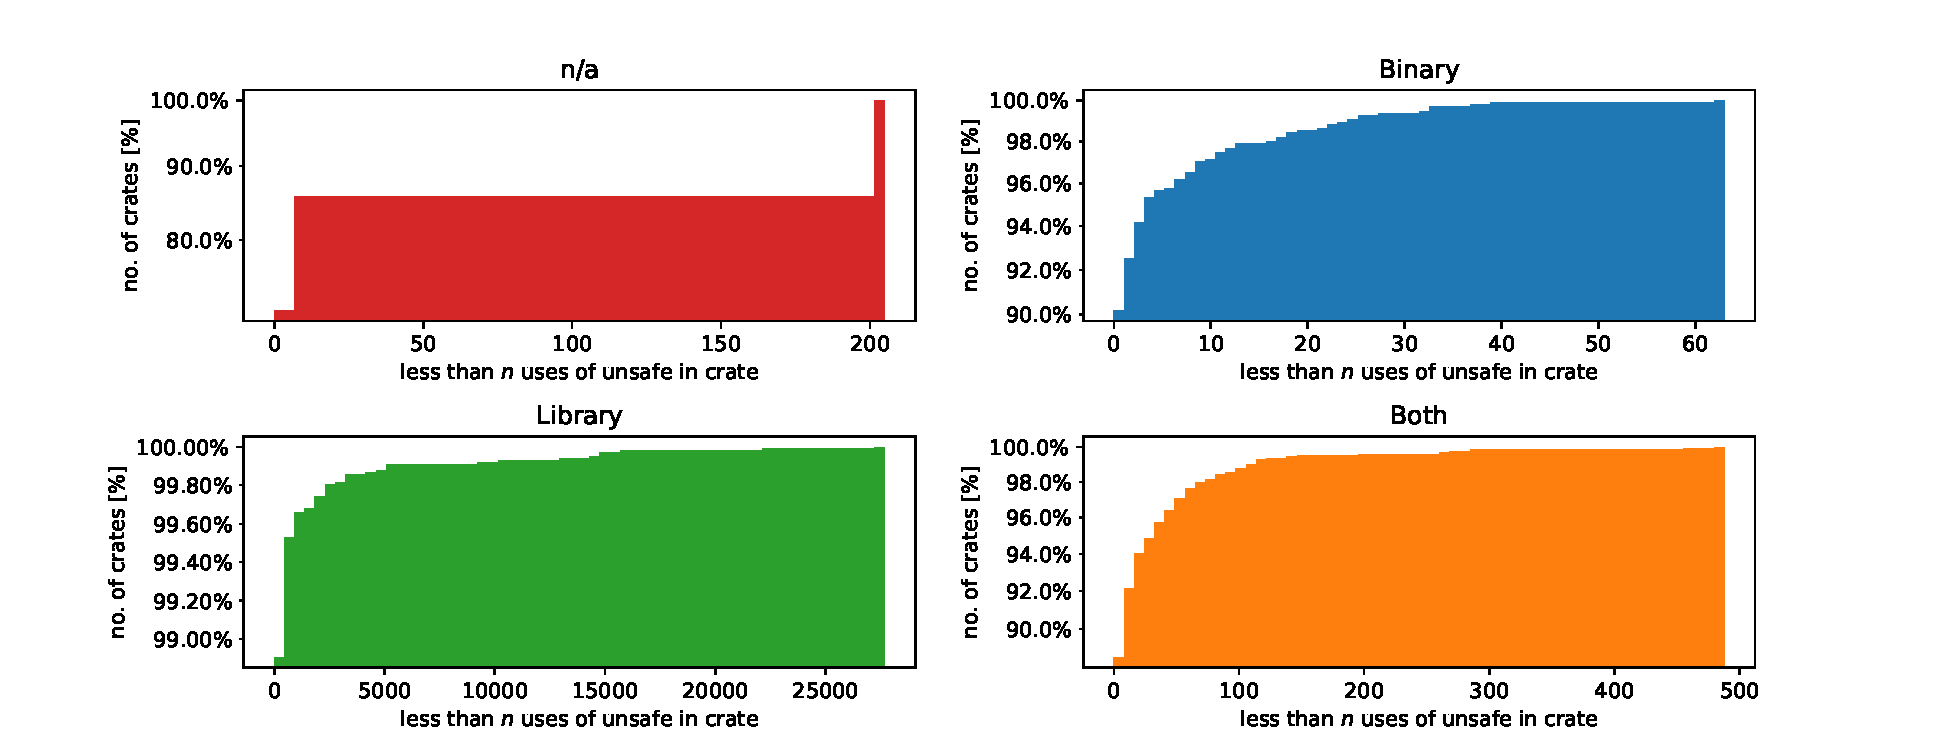
\includegraphics[width=0.99\linewidth, clip, trim={0.2cm 0.2cm 0.2cm 0.2cm}]{../unsafe_counts_by_crate_type.pdf}
	\caption{Cumulative, logarithmic histogram of the amount of \code{unsafe} uses in each category}
	\label{fig:unsafe-hist}
\end{figure}


\section{Mutability}

Finally we will check hypothesis \ref{enum:hypothesis-mut}, which asserts, that mutable variables and references are used pervasively in Rust.
This was checked by analysing the dataset for certain syntactical structures to infer mutability information about the following various AST items:
\begin{itemize}
	\item \textbf{Local Variable Definitions} can be tracked with high confidence. They occur in function bodies and take the form: \code{let mut a = <expr>}
	\item \textbf{Parameters}, which are considered immutable if they are passed as immutable references or owned. They take the syntactic form: \code{mut a: i32}
	\item \textbf{Function Definitions}, which are considered immutable, if all parameters considered immutable.
	\item \textbf{Arguments} are parts of a function call and can be arbitrary expression, which makes the tracking hard.
	\item \textbf{Function Calls}, which are considered immutable, if all arguments are considered immutable.
\end{itemize}

A total of around 52 million of these items were found in the dataset.

Figure~\ref{fig:mutabillity_by_category} shows the ratio of mutable to immutable items. For each syntactical category, the percentages are given relative to different objects:

\begin{enumerate}
  \item Total: number of occurrences
  \item Function: number of unique functions. I.e. 76.54\% of functions have a immutable parameter.
  \item File: number of unique files
\end{enumerate}


\begin{figure}[h]
	\centering
	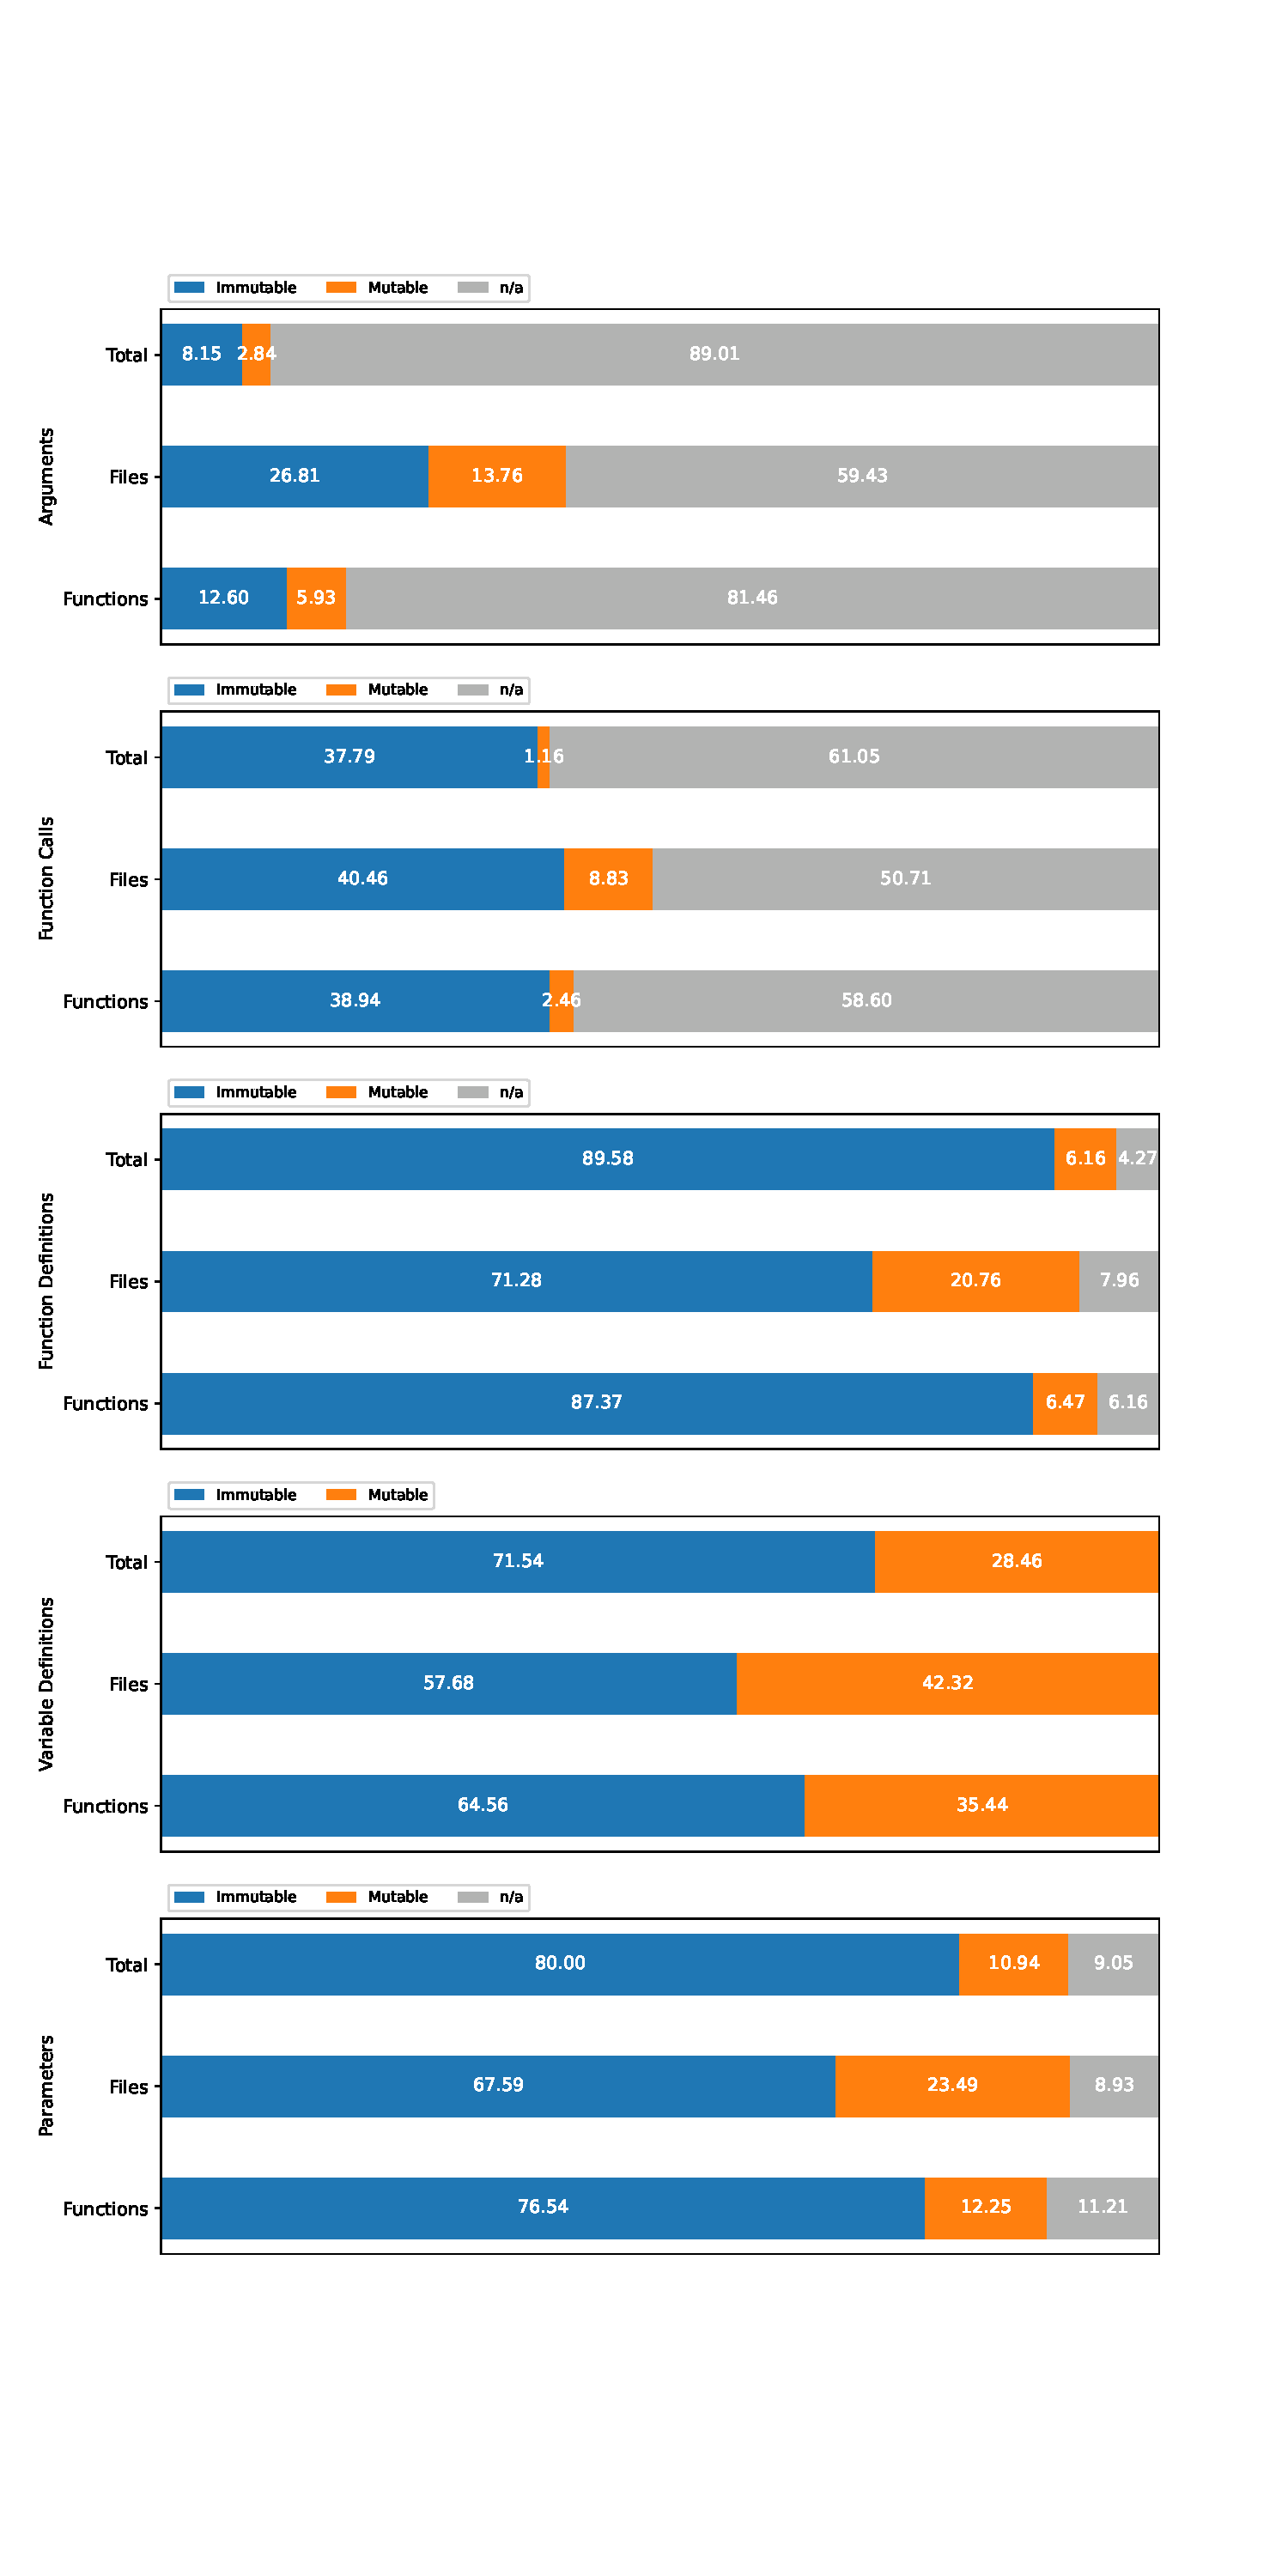
\includegraphics[width=0.9\linewidth, clip, trim={0.5cm 6cm 0.5cm 6cm}]{../mutability_by_category.pdf}
	\caption{Ratio of Immutable to Mutable Versions of Different AST Items. Items are Counted by Unique Occurrences}
	\label{fig:mutabillity_by_category}
\end{figure}

Unfortunately not there are some areas, where the syntactic analysis is not sufficient. Namely the analysis of function calls and arguments, which is mainly caused by the uncertainty of mutability of complex arguments.
Luckily the data from function definitions and parameters can complete the picture: About 80\% of parameters are immutable and between about 10 and 20\% of parameters are mutable. And less than 10\% of functions have mutable parameters at all.
When it comes to local variables, Rust users are more liberal in their use of mutability:
About 30\% of local variables are defined mutable.

For verification this means, that the use of mutability is wide spread. Especially local variables are often mutable and should therefore a verification system should try to minimize the effort for the user. Mutable parameters are less common, but still need to be accounted for in verification.

\section{Conclusions}

For this thesis the following conclusion can be drawn:

\begin{itemize}
  \item Even though uses of \code{unsafe} are not rare, it is acceptable to ignore in favour of a simpler type system.
  \item Mutable variables are used very often and should therefore have very little associated specification effort.
  \item Mutable parameters are used less frequently justifying a higher specification effort, but their specification must still be possible.
\end{itemize}

\chapter{Foundations}

\section{Rust}


\paragraph{Aliasing XOR Mutabillity} The key behind Rusts type system is, that for every variable at every point during the execution, that variable is either aliased or mutable, but never both at the same time.

Rust accomplished this by introducing three types of access permissions for a variable, which are associated with every scope\footnote{In modern Rust, this model was generalized to cover more cases, but the idea is still valid}:
\begin{enumerate}
  \item The scope \textit{owns} the variable. This guarantees, that no other scope has access to any part of the variable and allows the scope to create references to (part of) the variable.
  \item The scope (immutably) \textit{borrows} the variable. This guarantees, that as long as the variable is used, its \textit{value will not change} and allows the scope to further lend the variable to other scoped.
  \item The scope \textit{mutably borrows} the variable. This guarantees, that there are no other active references to any part of the memory of the variable.
\end{enumerate}

A consequence of these rules it, that at any time, every piece of memory has a unique and compile-time known owner. There are no reference cycles.

This makes both aliasing as well as mutability quite tame:
If a variable is aliased, it must be immutable and as a result, represents just a value (like in pure functional languages).
If a variable is mutable, it can not be aliased and as a result, any effect of the mutation is well known and locally visible.

\paragraph{The Case for Rust as a Target Language}


Rust justifies a new approach to mutable verification, because it is possible to take advantage of guarantees provided by (safe) Rust's ownership system. 

Rust is split into two languages: safe and unsafe Rust. Like most type systems, Rust's type and ownership system is conservative, meaning any (safe) Rust program that type checks, will not crash due to memory safety or type errors. Unsafe Rust gives the programmer the ability to expand the programs accepted by Rust outside that known-safe subset.

In this thesis, we will only consider safe Rust, which is the subset of Rust most programmers interact with (see section \ref{ss:unsafe-rust}).

Rust features a few unusual design decisions that profoundly influence the design of verification systems for it. The following paragraphs will elaborate on this.


\paragraph*{Opaque Generics} Rust does not provide a way to check a generic parameter for its instantiation. This means that we cannot extract any additional information from a generic parameter \code{T}. A function from \code{T} to \code{T} can therefor only be the identity function.
Wadler \cite{wadler_theorems_1989} shows, that it is possible to derive facts about the behaviour of such polymorphic functions.

In contrast, languages with instance-of-checks allow an implementation of a polymorphic function to distinguish between different instances of the generic parameter, precluding this extensive reasoning.

\paragraph*{Explicit Mutable Access} A consequence of the ownership rules is, that a function can only mutate (part of) the state, that is passed to it as a parameter. There is no global state and there is no implicit access to an object instance. Thus any intention of mutating state must already be expressed in the function signature, which makes the specification of this mutation quite natural.

\paragraph*{What Rust does not solve} Even though Rust simplifies reasoning about mutability and aliasing of mutable data, Rust does not eliminate the need to reason about multiple references to mutable data. For example, Listing \ref{lst:alias-mut} shows how \code{cell}'s type is influenced by changes to \code{r}. This does not mean, that the ownership rule  \textit{mutability XOR aliasing} are broken: Even though both \code{cell} and \code{r} are mutable, but only one is active.

\label{lst:alias-mut}\begin{lstlisting}
let mut cell = 2;
let r = &mut cell;
r+= 1;
assert(cell, 2)
\end{lstlisting}

\section{Refinement Types}

\chapter{The MiniCorten Language}

Rust's main disadvantage as a target language it its size: There is a lot of syntax and semantics that would need to be accounted. A lot of it even incidental to the verification. To reduce the complexity and amount of work, that needs to be done, we will focus on a subset of Rust described in this section.

The goal is to remove as much incidental complexity as possible without compromising to the central topic of research: How to extend LiquidTypes to mutability under the presence of Rust's ownership model.

\section{Features}

This subsection will explain some of the key features of the Corten type system.
Corten is directly embedded in Rust using two macros. Firstly the macro \code{ty!} can be used in place of a Rust type and adds a predicate to the Rust type, that any inhabitant of that type must satisfy. For example, the type \code{ty!\{ v : i32 | v >= 0\}} stipulates, that a value of Rust type \code{i32} is positive. The second macro is \code{relax\_ctx!\{ ... \}} which will be explained in subsection \ref{subsec:atomic-updates}.

\label{subsec:mutable-references}\subsection{Mutable References}

The key difference to Refinement Type Systems for functional languages to Rust it the pervasive use of mutation. Therefore the most important feature of Corten it the support for mutation and also mutable references.

The problem with references is the possibility of interdependencies: If one variable is changed, it might effect wether another variable is typed correctly. In listing \ref{lst:mutation} the return value \code{a} is effected by changes done to a different variable \code{a}. Conservative approximation requires, that all possible effects must be tracked.

Corten can accurately track references by phrasing them as predicates. For example the expression \code{\&mut a} will be typed as \code{ty!\{ \_1 : \&mut b | \_1 == \&a \}} (where \code{b} is the Rust type of \code{a}). This is sensible, because in Rust's ownership system, \code{a} must be the unique owner of the memory belonging to \code{a}. 
A more involved example is given in the evaluation \ref{subsec:evaluation-complex-mutable-ref}

Corten has two ways of dealing with assignment to mutable references: If the reference destination is known, the destination's type will be updated with the assigned values type (i.e. strong update). If there are multiple possible reference destinations, Corten will require the assigned value to satisfy the predicates of all possible destinations (i.e. weak updates). This is a standard approach (For example \cite{kloos_asynchronous_2015}), but more precise in Rust: The set of possible destinations only grows, when it depends on the execution of an optional control flow path. This means most of the time, strong updates are possible and weak updates are only needed if the reference destination is actually dynamic (i.e. dependent on the execution) \footnote{It would also be possible to encode the path condition in the reference type, but this was decided against for the stated goal of simplicity for the user}


- importance of tracing return of mutable references

\begin{listing}[h]
  \begin{minted}{rust}
    fn client() -> ty!{ v: i32 | v == 4 } {
        let a = 2; let b = &mut a;
        *b = 0; // changes a's value
        let c = &mut b;
        **c = 4; // changes a's value
        a
    }
  \end{minted}
  \caption{Example demonstrating interdependencies between mutable references}
  \label{lst:mutation}
\end{listing}

\label{subsec:path-sensitivify}\section{Path Sensitivity}

Firstly, the type system is path sensitive, meaning that the type system is aware of necessary XXX that need to be passed for an expression to be evaluated. For example listing \ref{lst:max-path-sensitive} shows a function computing the maximum of its inputs. In the then branch, $a$ is only a maximum of $a$ and $b$, because the condition $a > b$ implies it. Corten will symbolically evaluate the condition and store it in its typing context.

\begin{listing}[h]
  \begin{minted}{rust}
    fn max(a : ty!{ av: i32 }, b: ty!{ bv: i32 })
        -> ty!{ v: i32 | v >= av && v >= bv} {
        if a > b {
          a as ty!{ x : i32 | x >= av && x >= bv }
        } else {
          b
        }
    }
  \end{minted}
  \caption{Function computing the maximum of its inputs; guaranteeing that the returned value is larger than its inputs}
  \label{lst:max-path-sensitive}
\end{listing}


- inference
- also with mutations


\label{subsec:strong-type-updates}\section{Strong Type Updates}

\begin{listing}[h]
  \begin{minted}{rust}
    fn strong_updates(b: ty!{ bv: i32 | bv > 0}) -> ty!{ v: i32 | v > 2} {
        let mut a = 2;
        a = a + b;
        a
    }
  \end{minted}
  \caption{Example of changes to \code{a}'s value effecting its type}
  \label{lst:strong-updates}
\end{listing}



\label{subsubsec:modularity}\subsection{Modularity}

For a verification system to be scalable, it needs to be able modularize a proof. Corten can propagate type information across function calls and by taking advantage of Rust's ownership system, it can do so very accurately. Listing \ref{lst:modular-calls} shows, how an incrementing function \code{inc} can be specified: \code{inc} signature stipulates, that it can be called with any \code{i32} (given the name \code{a1}) and will return a value \code{a2}, which equals \code{a1 + 1}. Only the signature of \code{inc} is necessary for the type checking of \code{client}. 

Notice, that all of the type information about \code{y} is preserved when \code{inc(x)} is called. There are no further annotations needed to type check this program. This is possible, because in safe Rust, any (externally observable) mutation done by a function must be part of the function signature. Corten expands on this, by enabling the user specify exactly how a referenced value is mutated.

\begin{listing}[h]
  \begin{minted}{rust}
    fn inc(a: &mut ty!{ a1: i32 => a2 | a2 == a1 + 1 }) {
      *a = *a + 1;
    }
    fn client(mut x: ty!{ xv: i32 | xv > 2 }) -> ty!{ v: i32 | v > 7 } {
      let mut y = 2;
      inc(&mut x); inc(&mut x);
      inc(&mut y)
      x + y
    }
  \end{minted}
  \caption{Example showing how Corten allows for accurate type checking in the presence of function calls }
  \label{lst:modular-calls}
\end{listing}



\label{subsec:mutual-reference}\section{Mutual Reference}

Complex mutation patterns often result in complex interdependencies. We deem it necessary to allow different types to refer to each other.\todo{why?}

\begin{listing}[h]
  \begin{minted}{rust}
      let sum = 0;
      let i = 0;
      
  \end{minted}
  \caption{Function computing the maximum of its inputs; guaraneeing that the returned value is larger than its inputs}
  \label{lst:mutual-reference}
\end{listing}

\label{subsec:atomic-updates}\section{Atomic Updates}

- relax ctx
- non-atomic might not be sufficient


\section{Syntax}

\todo{Call it CortenRust (after Weathering Steel)}
This subsection will introduce the syntax of MiniCorten, a language modelled after a simplified version of Rust, with the addition of refinement types.
To simplify the formal definitions and proofs, the language is restricted to ANF\todo{What does the abbrev stand for? XXX Normal Form}, meaning arguments of expressions must be variables. Note that the implementation does not have this restriction.

\begin{bnfgrammar}
  $program$ ::=
    $func\_decl$ * : function declaration
  ;;
  $func\_decl$ ::=
    $ident$( $param$ * ) -> $ty$ \{ $stmt$ \}
  ;;
  $param$ ::= $ident$ \ccolon  $ty$
  ;;
  $stmt$ ::=
    $expr$                                                : expression
    | let mut? $ident$ = $expr$                           : declaration
    | $ident$ = $expr$                                    : assignment
    | while ($expr$) \{ $stmt$ \}                         : while loop
    | relax\_ctx!\{ $pred$* ; ($ident$ \ccolon $ty$)* \}  : context relaxation
  ;;
  $expr$ ::=
    $ident$                                         : variable reference
    | $lit$                                         : constant
    | $expr$ + $expr$                               : addition
    | $ident$($ident$ *)                            : function call
    | if $expr$ \{ $stmt$ \} else \{ $stmt$ \}      : if expression
    | $stmt$; $expr$                                : sequence
    | * $ident$                                     : dereference
    | \& $ident$                                    : immutable reference
    | \&mut $ident$                                 : mutable reference
    | $expr$ as $ty$                                : type relaxation
  ;;
  $ty$ ::= ty!\{ $logic\_ident$ \ccolon $base\_ty$ \cmid $pred$ \} : refinement type
  ;;
  $pred$ ::=
    $ref\_pred$                                     : predicate for a reference type
    | $value\_pred$                                 : predicate for a value type
  ;;
  $ref\_pred$ ::=
    $logic\_ident$ = \& $ident$
    | $ref\_pred$ \cdisj $ref\_pred$         : mutable reference
  ;;
  $value\_pred$ ::=
    $logic\_ident$                : variable
  | $pred$ \&\& $pred$            : conjunction
  | $pred$ \cdisj $pred$          : disjunction
  | ! $pred$                      : negation
  ;;
  $base\_ty$ ::=
    i32                     : integer
    | unit                  : unit type
    | bool                  : boolean
    | \& $base\_ty$         : immutable reference
    | \&mut $base\_ty$      : mutable reference
  ;;
  $lit$ ::=
      0,1,...,n             : integer
    | true                  : boolean true
    | false                 : boolean false
    | ()                    : unit value
\end{bnfgrammar}

\section{Semantics}

The semantics are mostly standard. The main difference being that Rust and our simplified language enable most statements to be used in place of an expression. The value is determined by the last statement in the sequence. For example If-Expressions, sequences of statements and function all follow this rule: Their (return) value is determined by the last statement or expression in the sequence.

The semantics loosely based on Jung's MiniRust.

Another difference between Rust and MiniCorten is of course the addition of refinement types.

In terms of the formal description, the rules are similar to Pierce's \cite[p. 166f]{pierce_types_2002-3} Reference language. % Also: Semantik von progrmmiersprachen WhileT p.45
The main difference is, that in Rust, every piece of data has a unique, known owner. This fact makes the concept of locations redundant. Instead we treat $\code{ref } x$ as a value itself. The following definitions show the new execution rules.

\begin{definition}[Execution-State]
  The state of execution is given by $\sigma : \text{PVar} \to \text{Value}$. The set of function declarations is constant and given by $\Sigma : \text{Fn-Name} \to ((\text{Arg}_1, \dots, \text{Arg}_n), \text(ReturnValue))$
\end{definition}

\begin{definition}[Small-Step Semantics of MiniCorten: $\tuple{e}{\sigma} \leadsto \tuple{e'}{\sigma'}$]


\begin{gather*}
  \inferrule*[left=SS-Assign]
    {\star}
    {x = v \mid \sigma \leadsto \code{unit} \mid \sigma[x \mapsto v]}
  \inferrule*[left=SS-Assign-Inner]
    {t \mid \sigma \leadsto t' \mid \sigma'}
    {x = t \mid \sigma \leadsto x = t' \mid \sigma'}
  \\
  \inferrule*[left=SS-Decl]
    {\star}
    {\tuple{\code{let } x = v}{\sigma} \leadsto \tuple{unit}{\sigma[ x \mapsto v]}}
  \\
  \inferrule*[left=SS-Deref]
    {\sigma(x) = v}
    {* \code{ref } x \mid \sigma \leadsto v \mid \sigma}
  \inferrule*[left=SS-Deref-Inner]
    {t \mid \sigma \leadsto t' \mid \sigma'}
    {* t \mid \sigma \leadsto * t' \mid \sigma'}
  \\
  \inferrule*[left=SS-Ref-Inner]
      {t \mid \sigma \leadsto t' \mid \sigma'}
      {\code{ref } t \mid \sigma \leadsto \code{ref } t' \mid \sigma'}
  \\
  \inferrule*[left=SS-Seq-Inner]
      {e_1 \mid \sigma \leadsto e_1' \mid \sigma'}
      {e_1; e_2 \mid \sigma \leadsto e_1', e_2 \mid \sigma'}
  \inferrule*[left=SS-Seq-N]
    {\star}
    {\code{unit}; e_2 \mid \sigma \leadsto e_2 \mid \sigma'}
  \\
  \inferrule*[left=SS-IF-T]
    {\sigma(x) = \code{true}}
    {\tuple{\code{if } x\ \{ e_t \} \code { else } \{ e_e \} }{\sigma} \leadsto \tuple{e_t}{\sigma}}
  \inferrule*[left=SS-IF-F]
    {\sigma(x) = \code{false}}
    {\tuple{\code{if } x\ \{ e_t \} \code { else } \{ e_e \} }{\sigma} \leadsto \tuple{e_e}{\sigma}}
  \\
  \inferrule*[left=SS-While]
    {\star}
    {
      \tuple{ \code{while } e_c\ \{\ e_b \}}{\sigma}
      \leadsto
      \tuple{ \code{if } e_c \{ e_b;  \code{while } e_c \{ e_b \} \} { \code{ else } } \{ \code{unit} \} }{\sigma}
    }
\end{gather*}

\end{definition}

\chapter{The Refinement Type System}

\section{Definitions}

\paragraph*{$P$} is the set of program variables used in rust program. Common names $a, b, c$
\paragraph*{$L$} is the set of logic variables used in refinement types. Common names: $\alpha, \beta$

\paragraph*{$\Gamma = (\mu, \Phi)$} is a tuple containing a function $\mu: P \to L$ mapping all program variables to their (current) logic variable and a set of formulas $\Phi$ over $L$. During execution of statements, the set increases monotonically

\paragraph*{$\tau$} is a user defined type $\{ \alpha : b \mid \varphi\}$. Where $\alpha$ is a logic variable from $L$, $b$ is a base type from Rust (like \texttt{i32}) and $\varphi$ is a formula over variables in $L$.

\paragraph*{Abbreviations}
We write:
\begin{itemize}
  \item  $\Gamma, c$ for $(\mu, \Phi \wedge c)$
  \item $\Gamma[a \mapsto \alpha]$ for $(\mu[a \mapsto \alpha], \Phi)$
\end{itemize}


\section{Expression Typing: $\Gamma \vdash e : \tau \Rightarrow \Gamma'$}

\begin{gather*}
  \inferrule*[left=Lit]
    {l \text{ fresh} \\ \text{base\_ty}(v) = b}
    {\Gamma \vdash v: \{ l : b \mid l \doteq v\} \Rightarrow \Gamma}
  %
  \\
  \inferrule*[left=Var]
    {\alpha \text{ fresh} \\ \mu(x) = \beta}
    {\Gamma = (\mu, \Phi)\vdash x : \{ \alpha : b \mid \beta \doteq \alpha \} \Rightarrow \Gamma}
  %
  \\
  \inferrule*[left=Var-Ref]
    {\Gamma \vdash y : \tau \\ \Gamma \vdash x : \{ \beta : \&b \mid \beta \doteq \&y \}}
    {\Gamma \vdash *x : \tau \Rightarrow \Gamma}
  %
  \\
  \inferrule*[left=If]
    {
      \Gamma \vdash \mu(x) : \text{bool} \Rightarrow \Gamma
      \\ \Gamma, \mu(x) \doteq \code{true} \vdash e_t : \tau \Rightarrow \Gamma'
      \\ \Gamma, \mu(x) \doteq \code{false} \vdash e_e : \tau \Rightarrow \Gamma'
    }
    {\Gamma \vdash \text{if } x \text{ then }e_t\text{ else } e_e : \tau \Rightarrow \Gamma'}
  %
  \\
  \inferrule*[left=While]
    {
      \Gamma_I, \mu(x) \doteq \code{true} \vdash s \Rightarrow \Gamma_I'
      \\ \Gamma_I', \mu(x) \doteq \code{true} \preceq \Gamma_I
    }
    {\Gamma_I \vdash \texttt{while } x \{ s \} \Rightarrow \Gamma_I,\mu(x) \doteq \code{false}}
  %
  \\
  \inferrule*[left=Seq]
    {
      \Gamma \vdash s_1 : \tau_1 \Rightarrow \Gamma'
      \\ \Gamma' \vdash \bar s : \tau \Rightarrow \Gamma''
    }
    {\Gamma \vdash s_1 ; \bar s : \tau \Rightarrow \Gamma''}
  %
  \\
  \inferrule*[left=Add]
    {
      \gamma \text{ fresh}
      \\ \mu(x_1) = \alpha
      \\ \mu(x_2) = \beta
    }
    {\Gamma \vdash x_1 + x_2 : \{ \gamma: b \mid \gamma \doteq \alpha + \beta \} \Rightarrow \Gamma}
  %
  \\
  \inferrule*[left=Decl]
    {
      \Gamma \vdash e :  \{ \beta \mid \varphi \} \Rightarrow \Gamma'
    }
    {\Gamma \vdash \code{let } x = e : \code{()} \Rightarrow \Gamma'[ x \mapsto \beta], \varphi}
  %
  \\
  \inferrule*[left=Assign]
    {\Gamma \vdash e : \{ \beta \mid \varphi \} \Rightarrow \Gamma'}
    {\Gamma \vdash x = e : \code{unit} \Rightarrow \Gamma' [x \mapsto \beta], \varphi}
  %
  \\
  \inferrule*[left=Assign-Strong]
    {
      \Gamma \vdash e : \{ \beta \mid \varphi \} \Rightarrow \Gamma'
      \\ \Gamma \vdash x: \{ \alpha : \& b \mid \alpha \doteq \&y\}
    }
    {\Gamma \vdash *x = e : \tau \Rightarrow \Gamma' [y \mapsto \beta], \varphi}
  %
  \\
  \inferrule*[left=Assign-Weak]
    {
      \Gamma \vdash e : \tau \Rightarrow \Gamma'
      \\ \Gamma' \vdash x: \{ \alpha : \& b \mid \alpha \doteq \&y_1 \vee \dots \vee \alpha \doteq \&y_n \} \Rightarrow \Gamma'
      \\ \Gamma' \vdash \tau \preceq \{ \beta_1 \mid \varphi_1 \}
      \\ \Gamma'[x \mapsto \beta_1], \varphi_1 \preceq \Gamma'
      \\\\ \dots
      \\\\
      \\ \Gamma' \vdash \tau \preceq \{ \beta_n \mid \varphi_n \}
      \\ \Gamma'[x \mapsto \beta_n], \varphi_n \preceq \Gamma'
      }
    {\Gamma \vdash *x = e : \tau \Rightarrow \Gamma'}
  %
  \\
  \inferrule*[left=Fn-Call]
    {
      \text{subst} = ...
      \\
      \\ (\mu[subst], \alpha \doteq \mu(a) \wedge \dots \wedge \varphi_{\alpha} \wedge\dots) \preceq (\mu, \Phi)
      \\ f : (\{ \alpha \mid \varphi_{\alpha} \} \Rightarrow \{ \alpha' \mid \varphi'_{\alpha} \}, \dots) \to \tau
    }
    {(\mu, \Phi) \vdash f(a, \dots, \&mut b, \dots) : \tau \Rightarrow (\mu[a \mapsto \alpha', \dots, subst^{-1}], \Phi \wedge \varphi'_{\alpha} \wedge \dots)}
  %
  \\
  \inferrule*[left=Intro-Sub]
    {
      \Gamma \vdash e : \tau
      \\ \Gamma \vdash \tau \preceq \tau'
    }
    {\Gamma \vdash e \texttt{ as } \tau': \tau'}
\end{gather*}

\section{Try: Statements $\Gamma \vdash s \Rightarrow \Gamma'$}

\begin{gather*}
  \inferrule*[left=If]
    {
      \Gamma \vdash \mu(x) : \text{bool} \Rightarrow \Gamma
      \\ \Gamma, \mu(x) \doteq \code{true} \vdash s_t \Rightarrow \Gamma'
      \\ \Gamma, \mu(x) \doteq \code{false} \vdash s_e \Rightarrow \Gamma'
    }
    {\Gamma \vdash \text{if } x \text{ then }s_t\text{ else } s_e \Rightarrow \Gamma'}
  %
  \\
  \inferrule*[left=While]
    {
      \Gamma_I, \mu(x) \doteq \code{true} \vdash s \Rightarrow \Gamma_I'
      \\ \Gamma_I', \mu(x) \doteq \code{true} \preceq \Gamma_I
    }
    {\Gamma_I \vdash \texttt{while } x \{ s \} \Rightarrow \Gamma_I,\mu(x) \doteq \code{false}}
  %
  \\
  \inferrule*[left=Seq]
    {
      \Gamma \vdash s_1 \Rightarrow \Gamma'
      \\ \Gamma' \vdash s_2 \Rightarrow \Gamma''
    }
    {\Gamma \vdash s_1 ; s_2 \Rightarrow \Gamma''}
  %
  \\
  \inferrule*[left=Decl]
    {
      \Gamma \vdash e :  \{ \beta \mid \varphi \}
    }
    {\Gamma \vdash \code{let } x = e  \Rightarrow \Gamma'[ x \mapsto \beta], \varphi}
  %
  \\
  \inferrule*[left=Assign]
    {\Gamma \vdash e : \{ \beta \mid \varphi \}}
    {\Gamma \vdash x = e \Rightarrow \Gamma' [x \mapsto \beta], \varphi}
  %
  \\
  \inferrule*[left=Assign-Strong]
    {
      \Gamma \vdash e : \{ \beta \mid \varphi \}
      \\ \Gamma \vdash x: \{ \alpha : \& b \mid \alpha \doteq \&y\}
    }
    {\Gamma \vdash *x = e \Rightarrow \Gamma [y \mapsto \beta], \varphi}
  %
  \\
  \inferrule*[left=Assign-Weak]
    {
      \Gamma \vdash e : \tau
      \\ \Gamma' \vdash x: \{ \alpha : \& b \mid \alpha \doteq \&y_1 \vee \dots \vee \alpha \doteq \&y_n \}
      \\ \Gamma \vdash \tau \preceq \{ \beta_1 \mid \varphi_1 \}
      \\ \Gamma[x \mapsto \beta_1], \varphi_1 \preceq \Gamma
      \\\\ \dots
      \\\\
      \\ \Gamma \vdash \tau \preceq \{ \beta_n \mid \varphi_n \}
      \\ \Gamma[x \mapsto \beta_n], \varphi_n \preceq \Gamma'
      }
    {\Gamma \vdash *x = e \Rightarrow \Gamma'}
  %
  \\
  \inferrule*[left=Fn-Call]
    {
      \text{subst} = ...
      \\
      \\ (\mu[subst], \alpha \doteq \mu(a) \wedge \dots \wedge \varphi_{\alpha} \wedge\dots) \preceq (\mu, \Phi)
      \\ f : (\{ \alpha \mid \varphi_{\alpha} \} \Rightarrow \{ \alpha' \mid \varphi'_{\alpha} \}, \dots) \to \tau
    }
    {(\mu, \Phi) \vdash \code{let res} = f(a, \dots, \code{\&mut} b, \dots) \Rightarrow (\mu[a \mapsto \alpha', \dots, subst^{-1}], \Phi \wedge \varphi'_{\alpha} \wedge \dots)}
\end{gather*}

\paragraph*{Expressions: $\Gamma \vdash e : \tau$}

\begin{gather*}
  \inferrule*[left=Lit]
    {l \text{ fresh} \\ \text{base\_ty}(v) = b}
    {\Gamma \vdash v: \{ l : b \mid l \doteq v\} }
  %
  \\
  \inferrule*[left=Var]
    {\alpha \text{ fresh} \\ \mu(x) = \beta}
    {\Gamma = (\mu, \Phi)\vdash x : \{ \alpha : b \mid \beta \doteq \alpha \} }
  %
  \\
  \inferrule*[left=Var-Ref]
    {\Gamma \vdash y : \tau \\ \Gamma \vdash x : \{ \beta : \&b \mid \beta \doteq \&y \}}
    {\Gamma \vdash *x : \tau }
  %
  \\
  \inferrule*[left=Add]
    {
      \gamma \text{ fresh}
      \\ \mu(x_1) = \alpha
      \\ \mu(x_2) = \beta
    }
    {\Gamma \vdash x_1 + x_2 : \{ \gamma: b \mid \gamma \doteq \alpha + \beta \} }
  %
  \\
  \inferrule*[left=Intro-Sub]
    {
      \Gamma \vdash e : \tau
      \\ \Gamma \vdash \tau \preceq \tau'
    }
    {\Gamma \vdash e \texttt{ as } \tau': \tau'}
\end{gather*}


\section{Function Declaration Type Checking}

Without loss of generality, we assume arguments are ordered by their type: First immutable / owner arguments and then mutable arguments.

When handling mutable references in parameters some sublteties need to be considered. The function can change both the referenced \textit{value} as well as the reference \textit{location}. To describe the referenced value is normally done using the $\{ \alpha \mid \alpha \doteq \&b\}$ syntax. The question arrises: If $\alpha$ was the logic variable for a parameter, what should be the analog for $b$? In contrast to local variables, there is no variable representing the referenced value for parameters. As seen in section \ref{subsec:mutable-references}, using the dereference operator would come with a lot of complications.
Instead we introduce $arg^i_n$, a special variable denoting the intial abstract value (i.e. stack location), that the mutable reference of argument $n$ points to. $i$ denotes the level of nesting: For the $n$th parameter with the Rust type \code{\&mut \&mut i32} we would generate $arg^1_n$ and $arg^2_n$.

\begin{gather*}
  \inferrule*[left=Fn-Decl]
    { (\{ a_1 \mapsto \alpha_1, b_1 \mapsto \delta_1 \}, \varphi^\alpha_1 \wedge \dots \wedge \delta_1 = arg^1_1 \wedge \varphi^\beta_1 \wedge \dots ) \vdash \bar s \Rightarrow \Gamma'
      \\ \Gamma' \vdash s_{res} : \tau_{res} \Rightarrow \Gamma''
      \\ \Gamma'' \vdash \tau_{res} \preceq \tau
      \\ \Gamma'' \preceq (\{\beta_1 \mapsto \gamma_1\}, \varphi^\gamma_1 )
    }
    {\code{fn } f(a_1 : \{ \alpha_1 \mid \varphi^\alpha_1 \}, \dots, b_1 : \{ \beta_1 \mid \varphi^\beta_1 \Rightarrow \gamma_1 \mid \varphi^\gamma_1\}) \to \tau \{ \bar s; s_{res} \}}
\end{gather*}

\section{Sub-Typing Rules: $\Gamma \vdash \tau \preceq \tau'$}

\[
  \inferrule*[left=$\preceq$-Ty]
    {\Phi \wedge \varphi'[\beta \triangleright \alpha ] \vDash \varphi}
    {\Gamma = (\mu, \Phi) \vdash \{ \alpha \mid \varphi\} \preceq \{ \beta \mid \varphi' \}}
\]

alternative (should be equivalent):

\[
  \inferrule*[left=$\preceq$-Ty-Alt]
    {
      \Gamma[f \mapsto \alpha], \varphi \preceq \Gamma[f \mapsto \beta], \varphi'
      \\ f \text{ fresh}
    }
    {\Gamma \vdash \{ \alpha \mid \varphi\} \preceq \{ \beta \mid \varphi' \}}
\]


\section{Sub-Context Rules: $\Gamma \preceq \Gamma'$}

\[
  \inferrule*[left=$\preceq$-Ctx]
    {
      \Phi'[\mu(\alpha) \triangleright \mu'(\alpha)\ \mid \alpha \in dom(\mu)] \vDash \Phi
      \\ dom(\mu) \subseteq dom(\mu')
    }
    {(\Phi, \mu) \preceq (\Phi', \mu')}
\]

In constrast to other refinement type systems, Corten allows types in the context to refer to one another.
For example a type specifications \code{a : \{ $\alpha$ : i32 | $\alpha$ > $\beta$\}, b:  \{ $\beta$: i32 | $\beta$ != $\alpha$\}} would be valid and result in the context $\Gamma = (\emptyset, \alpha \neq \beta \wedge \beta \geq \alpha)$. In the example $0$ is a subtype of \code{a}'s type as long as $\code{b} \geq 1$.

This means that types may need to be changed atomically.

\section{Soundness of the Type System}

As usual, we consider the three properties (see Pierce \cite[p. 95, p.167]{pierce_types_2002}) of a type system when assessing the correctness of MiniCorten:

\begin{definition}
  State Conformance: A state $\sigma$ is conformant with respect to a typing context $\Gamma = (\mu, \varphi)$ (written as $\sigma : \Gamma$), iff:
  $$\vDash \left(\bigwedge_{x \in \text{Var}} \mu(x) \doteq \sigma(x)\right) \to \varphi$$
   I.e. the a execution's value assignments imply the type refinements
\end{definition}

\begin{enumerate}
  \item Progress:
    \todo{need to show for program or term?}
    If $t$ is closed and well-typed, then $t$ is a value or $t \leadsto t'$, where $t'$ is a value.
  \item Preservation: If $\Gamma \vdash e : \tau \Rightarrow \Gamma$ and $e \leadsto e'$, then $\Gamma \vdash e' : \tau \Rightarrow \Gamma$
  \item Preservation of State Conformance
\end{enumerate}

The state conformance rule differs from the usual rule in two ways. Firstly we consider the runtime value instead of the runtime type. Secondly there needs to be one set of variable assignments that satisfies all predicates in $\Gamma$.

Because MiniCorten is based on Rust, we will assume, that progress, as well as preservation for the base-types. This includes preservation of type- and ownership-safety. Thus it is sufficient to prove, that assuming these properties hold, preservation of the refinement types is holds.


\begin{lemma}
  Preservation of State Conformance: If $\Gamma \vdash e : \tau \Rightarrow \Gamma'$, $\sigma : \Gamma$ and $\tuple{t}{\sigma} \leadsto \tuple{t'}{\sigma'}$, then  $\sigma' : \Gamma$
\end{lemma}


\begin{proof} Rule Induction over $\tuple{t}{\sigma} \leadsto \tuple{t'}{\sigma'}$
\begin{itemize}
  \item \textsc{Case SS-Assign}
    $\sigma' = \sigma[x \mapsto v]$. With rule inversion \textsc{Assign}: \code{unit} and post state: $\Gamma'[x \mapsto \beta], \varphi$ with $\Gamma \vdash e : \{ \beta \mid \varphi \}$.

    $e$ is a value, because of the requirement in \textsc{SS-Assign}. By rule inversion \textsc{Lit} over assumption $\Gamma \vdash v: \{ \beta \mid \varphi \} \Rightarrow \Gamma$: $\varphi = (\beta \doteq v)$

    $\mu'(x) = \beta$, $\sigma'(x) = v$ and induction hypothesis $\sigma : \Gamma$. Since $\mu'(x) \doteq \varphi(x) \to \varphi$ is trivially valid. XXXBanane gives us the goal.
  \item \textsc{Case Var}
\end{itemize}
\end{proof}

\begin{lemma}
  State Conformance is XXXBanane: If $\sigma : \Gamma$, $(\beta = v) \to \varphi$ then
    $\sigma[x \mapsto v] : \Gamma[x \mapsto \beta] \wedge \varphi$
\end{lemma}

\begin{proof}
  $$\vDash \left(\bigwedge_{x \in \text{Var}} \mu(x) \doteq \sigma(x)\right) \to \varphi$$
  ...?
\end{proof}

\section{Extensions}

\subsection{Records / \code{struct}s}
\subsection{Predicate Generics}

\chapter{Implementation}


- Type Aliases
- working without special compiler
- compiler plugin
- IDE
- HIR
- Location data (spans)
- Additional features
  - basic inference
  - no ANF

\chapter{Evaluation}

\section{Maximum using Path Conditions}



\section{Rephrasing builtins in terms of Refinement Types}

\paragraph*{panic}
\paragraph*{assert}

\label{subsec:evaluation-complex-mutable-ref}\section{Complex Mutable References}

\section{Proof of the Gauss Summation Formula}

\chapter{Related Work}

There currently does not exist an implementation of refinement types for Rust.

Relevant papers originate from two lines of work. Firstly additions to refinement types for mutability, asynchronous execution etc. and secondly other verification frameworks for Rust.

For example, Lanzinger \cite{lanzinger_property_2021} successfully adapted refinement types to Java, which allows the user to check, that property types described by java annotations hold true throughout the program. At this point in time, specification and verification is limited to immutable (\code{final}) data.

Kloos et al. \cite{kloos_asynchronous_2015} extended refinement types to mutable and asynchronous programs. The paper explores how changes to possibly aliased memory cells can be tracked throughout a OCaml program. For that purpose the types are extended by a set of requirements on memory objects, which track distinctness and refined types of these memory cells. In contrast to OCaml, Rust already guarantees that mutable memory is not aliased and in particular \textit{all mutable memory locations must be accessible by a variable name in the current context}, which offers substantial advantages in terms of simplicity to specification and verification of Rust programs.

Refinement types are also used in other applications. For example Graf et al. \cite{graf_lower_2020} use refinement types to check the exhaustiveness of pattern matching rules over complex (G)ADT types in Haskell. To check the exhaustiveness of patterns in Liquid Rust with ADTs may require similar approaches.

In terms of alternative verification approaches, Prusti\cite{astrauskas_leveraging_2019} is notable, because of their work on formalizing the full Rust semantics, including \code{unsafe}. Prusti is a heavy-weight functional verification framework for Rust; based on separation logic.

Alternative verification approaches also exists: For example RustHorn\cite{matsushita_rusthorn_2020} employs constrained horn clauses based verification to Rust. Particularity relevant for this thesis is the novel formalization for mutable references used in the paper. The authors stipulate that mutable references should be specified by a pre- and post-state from before a reference is borrowed to after it is returned.

The notion of Abstract Refinement Types that this thesis is based on is defined by Vazou et al. \cite{vazou_abstract_2013}. The basic idea is to allow the programmer to "refine" language types with predicates from a decidable logic. The type system has a notion of subtyping for refined types, where one type is a subtype of another if one predicate implies the other.

\section{Comparison to Flux}

\chapter{Conclusion \& Future Work}

\printbibliography

\end{document}